% !TEX TS-program = pdflatex
% !TEX encoding = UTF-8 Unicode

% This file is a template using the "beamer" package to create slides for a talk or presentation
% - Giving a talk on some subject.
% - The talk is between 15min and 45min long.
% - Style is ornate.

% MODIFIED by Jonathan Kew, 2008-07-06
% The header comments and encoding in this file were modified for inclusion with TeXworks.
% The content is otherwise unchanged from the original distributed with the beamer package.

\documentclass{beamer}

\mode<presentation>
{
  \usetheme{Malmoe}
  % or ...

  %\setbeamercovered{transparent}
  % or whatever (possibly just delete it)
}


\usepackage[english]{babel}
\usepackage{graphicx}
\usepackage{amssymb}
\usepackage{multicol,multirow,array}
\setbeamertemplate{navigation symbols}{}%remove navigation symbols
\setbeamertemplate{footline}
{
  \leavevmode%
  \hbox{%
  \begin{beamercolorbox}[wd=.4\paperwidth,ht=2.25ex,dp=1ex,center]{author in head/foot}%
    \usebeamerfont{author in head/foot}\insertshortauthor
  \end{beamercolorbox}%
  \begin{beamercolorbox}[wd=.6\paperwidth,ht=2.25ex,dp=1ex,center]{title in head/foot}%
    \usebeamerfont{title in head/foot}\insertshorttitle\hspace*{3em}
    \insertframenumber{} / \inserttotalframenumber\hspace*{1ex}
  \end{beamercolorbox}}%
  \vskip0pt%
}
\makeatletter
%\setbeamertemplate{footline}[frame number]
\setbeamertemplate{headline}{}

\title[Association Testing with X Chromosome Data] % (optional, use only with long paper titles)
{Association Testing with X Chromosome Data\\
An Application to the HCHS/SOL RBC Trait}

%\subtitle
%{Presentation Subtitle} % (optional)

\author[Caitlin McHugh, with Tim Thornton] % (optional, use only with lots of authors)
{Caitlin McHugh, with Tim Thornton}
% - Use the \inst{?} command only if the authors have different
%   affiliation.

\institute[University of Washington] % (optional, but mostly needed)
{
  Department of Biostatistics\\
  University of Washington
}
% - Use the \inst command only if there are several affiliations.
% - Keep it simple, no one is interested in your street address.

\date[Short Occasion] % (optional)
{13 March 2015}

% If you have a file called "university-logo-filename.xxx", where xxx
% is a graphic format that can be processed by latex or pdflatex,
% resp., then you can add a logo as follows:

% \pgfdeclareimage[height=0.5cm]{university-logo}{university-logo-filename}
% \logo{\pgfuseimage{university-logo}}

% If you wish to uncover everything in a step-wise fashion, uncomment
% the following command: 

%\beamerdefaultoverlayspecification{<+->}


\begin{document}

\begin{frame}
  \titlepage
\end{frame}

\begin{frame}{Outline}
\tableofcontents
 % You might wish to add the option [pausesections]
\end{frame}

\section{Gene G6PD}
\begin{frame}{Xq28, gene G6PD}
\begin{itemize}
\item There are known associations between red blood cell count (RBC) and X chromosome loci in the gene G6PD on Xq28. 
\item This finding was replicated in the SOL samples when performing association tests using a mixed linear model adjusting for autosomal effects.
\item We tested the X chromosome SNPs using a mixed linear model specifically accounting for X chromosome effects, and again replicated the finding.
\end{itemize}
\end{frame}

\section{Autosomal Model}
\begin{frame}{Sample Set and Covariates\footnote{these are as described in the working group previously}}
We include all individuals with non-missing outcome and covariates, exclude Asian outliers identified with PCA and additionally exclude samples with
\begin{itemize}
\item blood/lymph malignant tumor
\item bone cancer
\item pregnancy
\item chronic kidney disease
\item chemotherapy
\item \% blasts $>$5
\item \% immature granulocytes $>$5
\end{itemize}
Fixed effect covariates included are sex, age, center, and autosomal ancestry eigenvectors 1-5.\\
We include random effects of block group, household and autosomal kinship.
\end{frame}

\section{Autosomal Results}
\begin{frame}{Previous Variance Component Estimates, n=12,502}
\begin{table}[h!]
\centering
\begin{tabular}{ccc}
  \hline
& estimate & 95\% CI \\ \hline
block group & 0.00363 & (-0.00177, 0.00903)\\
household &0.04945 & (0.02113, 0.07777)\\
autosomal kinship &0.28473 &(0.23215, 0.33732)\\
environment & 0.66218& (0.60989, 0.71448) \\ \hline
\end{tabular}
\caption{Estimate (95\% CI) of the proportion variance for each of the components.}
\label{table:varComp}
\end{table}
\end{frame}

\begin{frame}{Previous Genome-Wide Assoc Test Results, n=12,502}
\centering
\begin{figure}
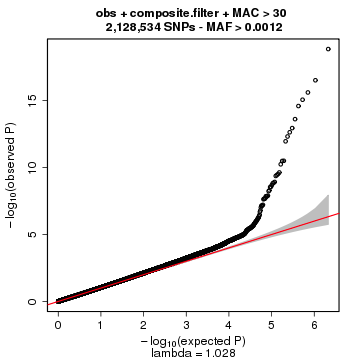
\includegraphics[height=4.6cm]{qq_obs_rbc.png}\\
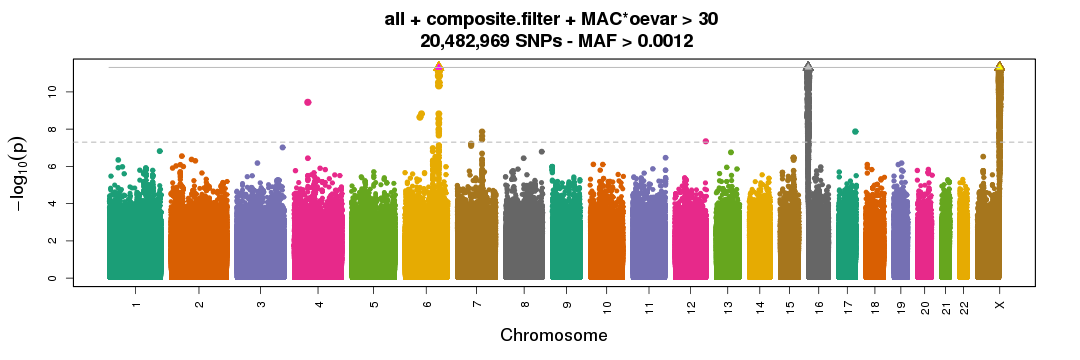
\includegraphics[width=11cm]{pval_manh_single_2014-08-12_04-43-43_316987.png}
\end{figure}
\end{frame}

\begin{frame}{Previous X Chr Assoc Test Results, n=12,502}
\centering
\begin{figure}
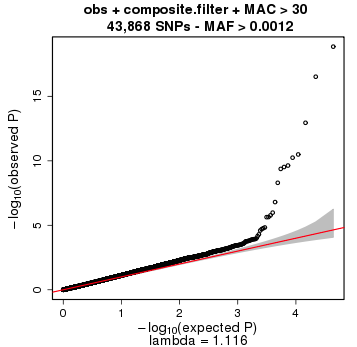
\includegraphics[height=4.6cm]{pval_qq_filtered_2015-02-27_11-37-52_auto_316987_v2.png}\\
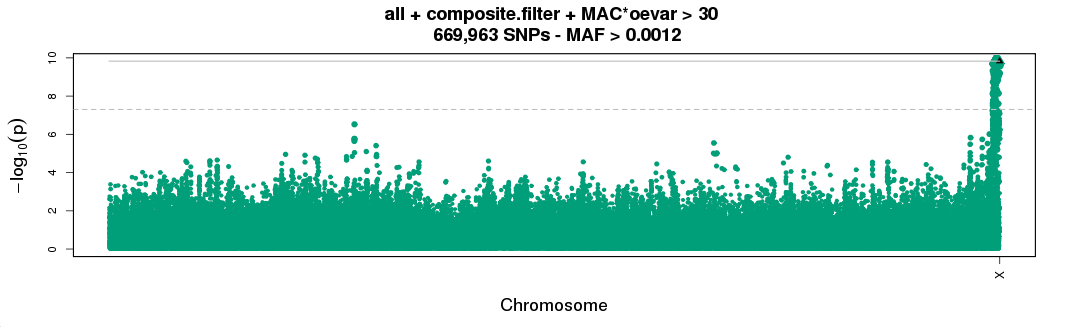
\includegraphics[width=11cm]{pval_manh_single_2015-02-27_11-37-52_auto_316987_v2.png}
\end{figure}
\end{frame}

\section{MLM-X Model}
\begin{frame}{MLM-X Model}
We include all individuals with non-missing outcome and covariates, exclude Asian outliers identified with PCA and additionally exclude samples with
\begin{itemize}
\item blood/lymph malignant tumor
\item bone cancer
\item pregnancy
\item chronic kidney disease
\item chemotherapy
\item \% blasts $>$5
\item \% immature granulocytes $>$5
\item \textbf{\textcolor{red}{an X chromosome anomaly}}
\end{itemize}
Fixed effect covariates included are sex, age, center, autosomal ancestry eigenvectors 1-5, and \textbf{\textcolor{red}{X chromosome ancestry eigenvectors 1-2}}.\\
We include random effects of block group, household, autosomal kinship and \textbf{\textcolor{red}{X chromosome kinship}}.
\end{frame}

\section{MLM-X Results}
\begin{frame}{MLM-X Variance Component Estimates, n=12,488}
\small
\begin{table}[h!]
\centering
\begin{tabular}{r|l||l}
  \hline
&MLM-X &Autosomal \\ \hline
%& estimate  (95\% CI)  & estimate (95\% CI) \\ \hline
block group & 0.00396 (-0.0016, 0.0095) & 0.00363 (-0.0018, 0.0090)\\
household &0.04950 (0.0209, 0.0781)& 0.04945  (0.0211, 0.0778)\\
autosomal kinship &0.28453 (0.2316, 0.3375) & 0.28473 (0.2322, 0.3373)\\
X kinship &0.02935 (0.0137, 0.0450) & \\
environment &0.63266 (0.5783, 0.6870) &  0.66218 (0.6099, 0.7145) \\ \hline
\end{tabular}
\caption{Estimate (95\% CI) of the proportion variance for each of the components.}
\label{table:varComp}
\end{table}
\end{frame}

\begin{frame}{MLM-X Assoc Test Results, n=12,488}
\centering
\begin{figure}
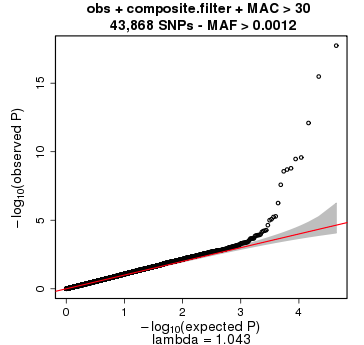
\includegraphics[height=4.6cm]{pval_qq_filtered_2015-02-27_11-42-21___316987_v2.png}\\
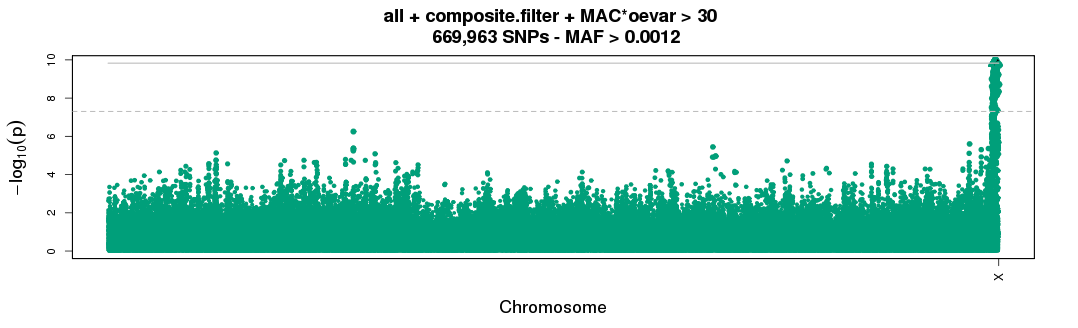
\includegraphics[width=11cm]{pval_manh_single_2015-02-27_11-42-21___316987_v2.png}
\end{figure}
\end{frame}

\begin{frame}{Index SNP rs1050828}
\begin{table}[ht]
\centering
\begin{tabular}{r|lll}
  \hline
 & Effect Size (SE) & Stat & p-value \\ 
  \hline
autosomal & 0.1314 (0.0145) & 81.9377 & 1.40447e-19 \\ 
MLM-X & 0.1300 (0.0148) & 76.8729 & 1.82321e-18 \\ 
 \hline
\end{tabular}
\end{table}
\end{frame}

\end{document}


